\documentclass[a4paper,10pt]{report}

\usepackage[utf8]{inputenc}
\usepackage[T1]{fontenc}
\usepackage[french]{babel}
%\usepackage[vlined, lined, linesnumbered, boxruled, french]{algorithm2e}
%\usepackage{xcolor,amsmath,amssymb}
%\usepackage[babel=true]{csquotes}
\usepackage{fancyhdr}
\usepackage{graphicx}
\pagestyle{fancy}
\usepackage{float}
\usepackage{setspace}
\usepackage{listings}
%%%%%%%%%%%%%%%% Lengths %%%%%%%%%%%%%%%%
\setlength{\textwidth}{15.5cm}
\setlength{\evensidemargin}{0.5cm}
\setlength{\oddsidemargin}{0.5cm}

\setlength{\voffset}{-.7in}
\setlength{\hoffset}{-.1in}
\setlength{\textheight}{24.7cm}

\renewcommand*\thesection{\arabic{section}}
%%%%%%%%%%%%%%%% Variables %%%%%%%%%%%%%%%%
\def\projet{1}
\def\titre{Projet Réseau}
\def\groupe{4}
\def\equipe{Anguille Sous Roche}
\def\others{Victor Dury, Antoine Pitaud, Reda Boudjeltia, Darius Matboo, Yoann Janvier}
\newtheorem{preuve}{\textit{Preuve }}
\begin{document}
\fancyhfoffset{0cm}{}
%%%%%%%%%%%%%%%% Header and footer %%%%%%%%%%%%%%%%
\noindent\begin{minipage}{0.98\textwidth}
\vskip 0mm
\noindent
    \begin{center}    { \begin{tabular}{p{4.5cm}}
        \centering \bfseries
                   {\itshape \titre} \\

    \end{tabular}} \\
    \hfill

    \fbox{\begin{tabular}{l}
        {~\hfill \bfseries \sffamily Groupe  \groupe\ - \'Equipe \equipe
          \hfill~} \\[2mm]
        Codeurs : \others
    \end{tabular}}
    \end{center}
    \vskip 4mm




    \vskip 1mm
\end{minipage}

\lhead{ Projet Réseau}
\chead{}
\rhead{Groupe \groupe \hspace{1mm}- Equipe \equipe}

\lfoot{ENSEIRB-MATMECA}
\cfoot{}
\rfoot{Semestre 8 2014-2015}

%%%%%%%%%%%%%%%% Main part %%%%%%%%%%%%%%%%
%\begin{doublespace}
\vskip 5cm
\begin{figure}[!h]
\centering

\includegraphics[scale=0.5]{inp.jpg}
\end{figure}

\tableofcontents

\newpage
\section{Introduction}
Ce projet nous propose d'implémenter un programme qui simulera un aquarium sur plusieurs écrans. Chaque écran devra afficher les poissons présents sur le noeud qu'il représente. En effet l'aquarium est géré avec l'aide d'un graphe, chaque écran représente un noeud et les poissons peuvent bouger dans tout l'aquarium et donc changer de noeud. \\
Ce projet à une architecture client-serveur centralisée, le serveur effectuera tous les calculs et transmettra ensuite les informations aux différents clients et affichages.\\
L'utilisateur doit saisir différentes commandes dans les consoles du serveurs et des clients qui lui permettrons de réguler plusieurs paramètres.  Ansi le serveur laisse la possibilité de gérer le graphe grâce à sa console alors que les consoles clients permettent de gérer la population de poissons présente dans l'aquarium.\\
Chaque client est lié à un noeud du graphe, il ne peut y avoir plus de clients que de noeuds et chaque noeud peut être lié à seulement un client.\\
Bien que les langages ne sont pas réellement imposés, un langage objet doit être utilisé pour l'interface client alors que le serveur doit être codé en C.


\section{Mode utilisateur}
Lors du lancement du programme ni le graphe ni l'aquarium ne sont définis, c'est l'utilisateur qui rentrera des commandes capables de gérer le graphe et les affichages.
\subsection{Console serveur}
\label{sec:console}
La console serveur permet de créer un graphe et de le modifier tout au long de l'utilisation. Certaines actions sont possibles :
\begin{itemize}
\item Charger un graphe à partir d'un fichier avec la commande \textit{load <path>}
\item Afficher un graphe déjà chargé avec la commande \textit{show}
\item Ajouter une arête entre deux noeuds avec la commande \textit{add link <$noeud_1$> <$noeud_2$>}
\item Supprimer une arête entre deux noeuds avec la commande \textit{del link <$noeud_1$> <$noeud_2$>}
\item Supprimer un noeud avec la commande \textit{remove <noeud>}
\item Sauvegarder le graphe mémoire dans un fichier avec la commande \textit{save <path>}
\end{itemize}

Bien que l'utilisateur puisse modifier le graphe en supprimant des noeuds ou arêtes, il ne peut ajouter un noeud. En effet le graphe devra toujours être défini dans un fichier de configuration qu'il faudra charger au début du programme.
Le fichier de configuration doit suivre un modèle afin d'être parsé correctement par le programme. \\

 \noindent graph Aquarium \{\\
    \indent n1 [label="N1"];\\
    \indent n2 [label="N2"];\\
    \indent n3 [label="N3"];\\
    \indent n4 [label="N4"];\\
    \indent n1 -- n2 [label="3"];\\
    \indent n1 -- n3 [label="2"];\\
    \indent n2 -- n4 [label="1"];\\
    \indent n3 -- n4 [label="4"];\\
\} \\
\label{the_label}
Ce format définit un graphe ayant 4 noeuds et 4 arêtes.

\subsection{Console client}
La console client permet de gérer la population de poissons présents dans l'aquarium. Certaines actions sont possibles:
\begin{itemize}
\item Avoir le statut du client avec la commande \textit{status}
\item Ajouter un poisson dans l'aquarium avec la commande \textit{addFish  <type> at <$depart_x$>x<$depart_y$>, <$cadre_x$>x<$cadre_y$>  <routineDeplacement>}

\item Supprimer un poisson avec la commande \textit{delFish <name>}
\item Lancer la routine de déplacement avec la commande \textit{startFish <name>}
\item Avoir les informations  concernant les poissons présents dans le noeud correspondant au client avec la commande  \textit{getFishes}
\item Avoir les informations  concernant les poissons présents dans le noeud correspondant au client en continue avec la commande \textit{getFishesContinuously}
\item Demander une déconnexion avec \textit{log out}
\end{itemize}

Il n'y a aucun poisson présent dans l'aquarium au démarrage du programme, c'est l'utilisateur qui devra créer chaque poisson s'il veut donner un peu de vie à son aquarium.


\section{Gestion du graphe}

\indent Comme vu auparavant, l'utilisateur devra avoir la possibilité de gérer un graphe, et associer chaque noeud du graphe à un aquarium. Par conséquent, nous avons implémenté un parseur de commandes permettant à l'utilisateur de charger un graphe, puis d'ajouter ou de retirer des arêtes à ce graphe, de lui retirer des noeuds, de pouvoir l'afficher ou bien simplement de quitter le programme.\\ Pour pouvoir faire cela, nous avons utilisé la bibliothèque $GraphViz$, et implémenté les commandes suivantes:\\
\begin{itemize}
\item Afin de charger le graphe (le graphe doit être placé dans un fichier séparé, et doit avoir le format défini en~\ref{the_label}), l'utilisateur devra écrire la commande \textit{load <path>}. Cette commande est reconnue grâce à la fonction de $GraphViz$: $g = agread(graph\_file, NULL)$.
\item Afin de retirer un noeud du graphe, la commande à entrer est: \textit{remove <noeud>} correspondant à la fonction $agdelete(g, ntmp)$, avec ntmp le noeud en question, et g le graphe déjà chargé.
\item Pour afficher le graphe, l'utilisateur fera simplement appel à la commande \textit{show}, et le parseur effectuera $agwrite(g, stdout)$.
\item Pour ôter une arête entre deux noeuds, la commande est: \textit{del link<$n_1$ $n_2$}, avec $n_1$ et $n_2$ le label des deux noeuds en question. Grâce à ce label, les deux noeuds sont retrouvés et sont respectivement placés dans les variables $tmp1$ et $tmp2$. \\Puis, la fonction $agdeledge(g, agedge(g, tmp1, tmp2, NULL, FALSE))$,  s'occupe de retirer l'arête. L'argument FALSE permet de ne pas créer l'arête si elle n'existe pas.
\item Pour ajouter une arête entre deux noeuds, l'utilisateur doit écrire \textit{add link $n_1$ $n_2$}. Les deux noeuds sont à nouveau placés dans les variables $tmp1$ et $tmp2$, puis le parseur appelle la fonction $agedge(g, tmp1, tmp2, NULL, TRUE)$.
\end{itemize}
\section{Un aquarium et des poissons}

\subsection{Les poissons}

\indent La structure poisson est caractérisée par: \\
\begin{itemize}
\item Un entier permettant d'identifier le poisson.
\item Une chaîne de caractères, son nom.
\item Une chaîne correspondant à l'espèce du poisson.
\item Une chaîne correspondant au label du noeud dans le graphe où il est placé.
\item Une chaîne correspondant décrivant la routine de déplacement que le poisson suivra pour arriver à sa position de destination.
\item Une coordonnée décrivant la position actuelle du poisson.
\item Une coordonnée décrivant les dimensions du rectangle dans lequel il lui est permis de naviguer.
\item Une coordonnée décrivant la position de destination du poisson.
\item Un entier correspondant au temps nécéssaire pour arriver à sa position de destination.
\end{itemize}
Cette structure poisson est reliée à une structure aquarium contenant tous les poissons.

\subsection{L'aquarium}
\indent Un aquarium se doit d'être un conteneur de poissons et englober le graphe. Nous avons ainsi créé une structure aquarium définie par un tableau de poissons, un graphe, et le nombre de poissons qui facilite le parcours du tableau.


\subsection{Les actions permises}

\indent L'utilisateur est maître de la population de l'aquarium. Il a le pouvoir d'ajouter, de pêcher, ou d'activer un déplacement pour un poisson. Le serveur quant à lui le tient informé des caractéristiques de chacun des poissons lorsque la requête est demandée via les méthodes $getFishes$, $getFishesContinuously$ et $status$.

\subsubsection{Les messages reçus du serveur}
\indent Le serveur reçoit des messages de la part des clients connectés, correspondants aux commandes effectuées sur les poissons à laquelle le serveur ajoute le numéro du noeud demandant la requete, sous la forme de chaînes de caractères. Afin de comprendre le message, un parseur décompose la chaîne en un tableau de chaînes divisant les mots du message séparés par un espace. Ainsi, le pointeur vers la première case du tableau nous renseigne sur l'action à effectuer, et ainsi sur la fonction à appeler. Les paramètres des fonctions sont contenues dans la chaînes.

\subsubsection{Créer un nouvel aquarium}

\indent La méthode $struct$ $aquarium$ $new\_aquarium(Agraph\_t*)$ est le constructeur de la structure aquarium. Le seul paramètre de cette fonction permettra de lier le graphe à l'aquarium. Puisque le graphe peut être modifié par l'utilisateur tout au long de la vie du processus, un pointeur est nécessaire pour une synchronisation entre l'aquarium et le graphe. \\
\indent Ainsi, nous allouons l'espace nécessaire pour une structure aquarium, puis nous plaçons le graphe dans la structure et nous initialisons son nombre de poissons à 0.

\subsubsection{Ajouter et Enlever un poisson}

\indent Afin d'ajouter un poisson, le serveur nous communique directement la commande du client concaténée avec le label du noeud correspondant au client. \\Ensuite, la méthode $int$ $addfish$($char*$,  $struct$ $aquarium*)$ décompose le message reçu. Un poisson est créé, et les informations contenues dans le message servent à initialiser le nouveau poisson demandé par l'utilisateur. Enfin, une fonction $add\_aqua$ permet d'ajouter réellement le poisson au tableau de poissons de la structure aquarium. \\
\indent Le retrait d'un poisson se fait après le parcours dans l'aquarium qui cherchera le poisson dont le nom est renseigné par l'utilisateur. Les champs des différentes structures sont mises à jour.

\subsubsection{Demande d'informations}
L'utilisateur peut demander des informations sur les poissons à tout moment. Plusieurs commandes sont disponibles, $status$, $getFishes$ et $getFishesContinuously$.\\
Une fonction $status$ permet de répondre à la commande du même nom. Cette fonction parcourt simplement l'aquarium principal et compare l'$id\_view$ de chaque poisson et celui renseigné dans le message.\\
 Lorsqu'un poisson a un $id\_view$ égale à celui indiqué, son nom est récupéré dans une chaine de caractères. $status$ renvoie alors la chaine resultant de la concaténation du nom de chaque poisson présent dans la vue demandée.\\
Une fonction $getFishes$, de la meme manière que $status$, renvoie des informations sur les poissons présents sur la vue courante.
Les informations renvoyées sont cependant bien plus précises que le seul nom renvoyé par $status$. A plus long terme ce sont les informations contenues dans cette réponse du serveur à la demande $getFishes$ qui permettront au programme d'affichage d'actualiser les positions et états de chaque poisson.\\
La demande $getFishesContinuously$ n'est en réalité qu'un appel continu à $getFishes$. C'est alors le contrôleur principal qui lancera un thread executant cette routine.

%\section{La commande}
%\input{commande}

\section{Le contrôleur}

\subsection{le serveur tcp}

\indent Parmi les différentes parties du controleur, on trouve ce que nous avons baptisé le serveur tcp.
Ce dernier prend en charge les communications entre le programme qui gère l'aquarium et le client.\\
\indent Lors d'une requête du client, le serveur tcp va vérifier la validité de la requête et appeler les fonctions correspondantes.
Dans le cas d'un \textit{getFishescontinously},
il crée un thread actif en parallèle de son thread principal qui appelle tout le temps la fonction \textit{getFishes}.

\begin{figure}[!h]
\caption{\label{handlers} Diagramme de séquences}
\begin{center}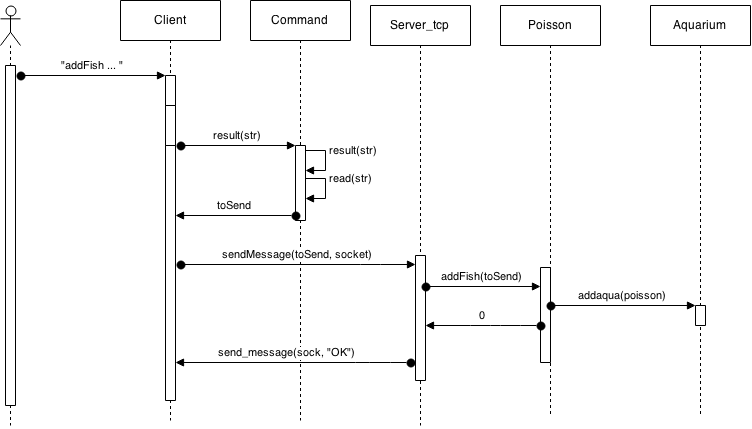
\includegraphics[scale=0.5]{Diagram}\end{center}
\end{figure}

D'autre part, le fonctionnement de cette partie est basée sur une simple aborescence de threads parmis lesquels nous
trouvons celui qui attend des requêtes à executer, et celui qui envoie les informations afin de rafraichir
l'aquarium du coté du client. Chacun des threads qui gère les requetes  est créé lors de l'acceptation
d'un client et est propre au client qui à pour identifiant le numéro de la socket qu'il utilise avec le serveur.

\begin{figure}[!h]
\caption{\label{handlers} Structure des clients côté serveur}
\begin{center}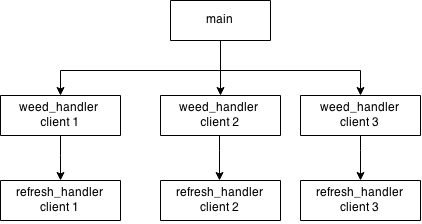
\includegraphics[scale=0.8]{thread}\end{center}
\end{figure}


Ainsi, lors d'une demande de deconnexion, le client demande à se déconnecter à l'aide de la requête \textit{exit},
le serveur reçoit le message et envoie la confirmation de déconnexion, fait un join de tous les threads et kill
et aussi éventuellement celui qui permet le rafraichissement, et fini par fermer la socket.
Néanmoins, meme si le client est déconnecté le serveur reste actif et attend d'autres clients potentiel,
via une boucle while munie d'une fonction accept propre au protocole tcp.

\section{Partie controleur de la vue}

\subsection{Le prompt client}

\indent Pour ce projet, le client doit pouvoir, comme l'a été mentionné précédemment saisir des commandes au niveau du prompt client.
Le client a aussi de son côté une interface graphique.
Il faut donc pouvoir mettre dans un thread à part la saisie de commande afin de ne pas bloquer le tout.

\subsection{Le parsing de commandes saisies}

\indent Le client instancie donc une classe Commande.java qui permet de vérifier que les commandes
saisies du côté client sont bien les bonnes. Cette classe fait essentiellement du parsing de commandes
en suivant le cahier des charges du projet. Il faut savoir que les commandes éronées ne sont jamais envoyées au serveur. Seules des commandes
valides sont envoyées afin de ne pas surcharger inutilement les demandes au serveur.

\subsection{Le traitement des commandes reçues}

\indent Un peu d'une même façon, le client va en même temps instancier une classe CommandReceived.java
pour pouvoir traiter les commandes reçues. Un parseur de string est utilisé afin de déclencher des actions selon les ordres. On admet
ici que les commandes reçues sont toujours correctes.\\
Cette classe possède un attribut view, construit par référence, afin de pouvoir declencher des méthodes de la vue du client, afin d' actualiser
l'aquarium selon les commandes fournies.

\subsection{Le client}

\indent La classe client est instanciée par un Main. Elle a plusieurs attributs nécessaires à la communication avec le serveur.
On a donc un attribut socket, un buffer pour lire et envoyer sur le socket, une vue pour instancier un aquarium
et un fichier de configuration pour lire les information nécessaires à l'établissement de la connexion avec le serveur (port et adresse). \\Nous avons aussi comme nous l'avons dit plus haut, un instance de Command et CommandReceived afin de parser
et effectuer la gestion des commandes.\\
De plus nous utilisons un scanner pour récupérer les commandes saisies par l'utilisateur
dans le prompt client.\\
Cette classe possède plusieurs threads. En effet, il faut pouvoir ne pas bloquer la console en écoutant sur le serveur. De plus le scan de
la console est bloquant aussi. Il faut donc l'isoler.\\
Enfin il y a deux méthodes importantes qui permettent de recevoir sur le socket, et
aussi de pouvoir envoyer au serveur les commandes voulues : ce sont $send_message$ et $rec_message$.\\
Le client va donc faire deux actions
et ce en continu : scanner la console à la recherche d'ordres, et obéir au serveur en écoutant sur le socket.


\section{Partie Affichage}
Concernant l'affichage en lui-même, il a fallu découper cet affichage en plusieurs fichiers afin d'obtenir de clair. Les fichiers sont les suivants :
\begin{itemize}
\item{\textbf{Entity.java :} Qui comporte toputes les informations nécessaires à la description d'un poisson}
\item{\textbf{Fish.java : }Qui se charge de déssiner les poissons sur l'aquarium grâce aux informations de la classe précédente}
\item{\textbf{Aquarium.java : }Qui se charge de peindre l'aquarium et d'y placer les différents poissons décrits par la classe précédente}
\item{\textbf{View.java : }Qui se charge de gérer l'affichage dans son ensemble et de le rafraîchir}
\end{itemize}
Nous allons vous présenter un peu plus en détails ces différentes classes.
\subsection{Le modèle Poisson}
Chaque poisson possède les informations suivantes :
\begin{itemize}
\item{Des coordonnées x et y, qui correspondent à la position d'un poisson en pixels sur l'aquarium}
\item{Un nom, qui correspond à celui que lui donne l'utilisateur lors de l'ajout de celui-ci}
\item{Un type, qui permet de charger l'image correspondante lors de l'affichage si elle existe sinon une image par défaut}
\item{Des entiers représentant la longueur et la largeur en pixels du carré d'affichage de ce poisson qui sont rentrés par l'utilisateur lors de son ajout}
\end{itemize}
Ainsi grâce à ces informations contenues dans la classe \textit{Entity.java}, nous sommes capables de décrire entièrement un poisson de manière statique.


\subsection{Dessin d'un poisson}
Le dessinage d'un poisson se fait depuis la classe \textit{Fish.java} grâce aux informations receuillies de la classe \textit{Entity.java}. Cette classe est censée dessiner un composant sur l'aquarium et possède donc un lien "est-un" avec la classe \textit{JComponent}. Chaque dessin de poisson se doit d'être fidèle à la représentation attendue et possède ainsi les attributs suivants :
\begin{itemize}
\item{Des coordonnées x et y afin de l'afficher correctement sur l'aquarium}
\item{Un poissonn afin de pouvoir mettre à jour sa position sur l'écran}
\item{Une image, qui correspond à l'attribut type de la classe \textit{Entity.java}}

\end{itemize}

Le poisson peut ainsi être dessiné avec les bonnes caractéristiques tout en sachant si ce dernier a été lancé ou non.

\subsection{Dessin de l'aquarium}

Chaque aquarium quant-à lui, se charge de s'afficher et donc "est-un" \textit{JPanel}. Il se doit également de "coller" tous les dessins de poissons qui se trouvent dans cet auqarium.
\newline Ainsi un aquarium possèdera les attributs suivants :
\begin{itemize}
\item{Deux entiers correspondant à la taille de l'aquarium en pixels}
\item{Une couleur}
\item{Une liste de dessins de poissons}
\end{itemize}

Cette classe se charge en autre d'ajouter, supprimer les dessins de poissons de sa liste mais aussi de mettre à jour sa liste de poissons lors d'un rafraîchissement.

\subsection{Affichage global}

Enfin l'affichage de l'aquarium est géré depuis la classe \textit{View.java} qui se charge d'instancier un aquarium et de passer les ordres d'ajout, de suppression et de lancement d'un poisson à l'aquarium.


\section{Utilisation et réalisation}



\subsection{Utilisation}

\indent Confer README.txt

\subsection{Exemple de rendu}

Voici sur la figure \ref{exempleAqua} la fenêtre que pourra obtenir un client:

\begin{figure}[!h]
\caption{\label{exempleAqua} Exemple d'un aquarium à trois poissons}
\begin{center}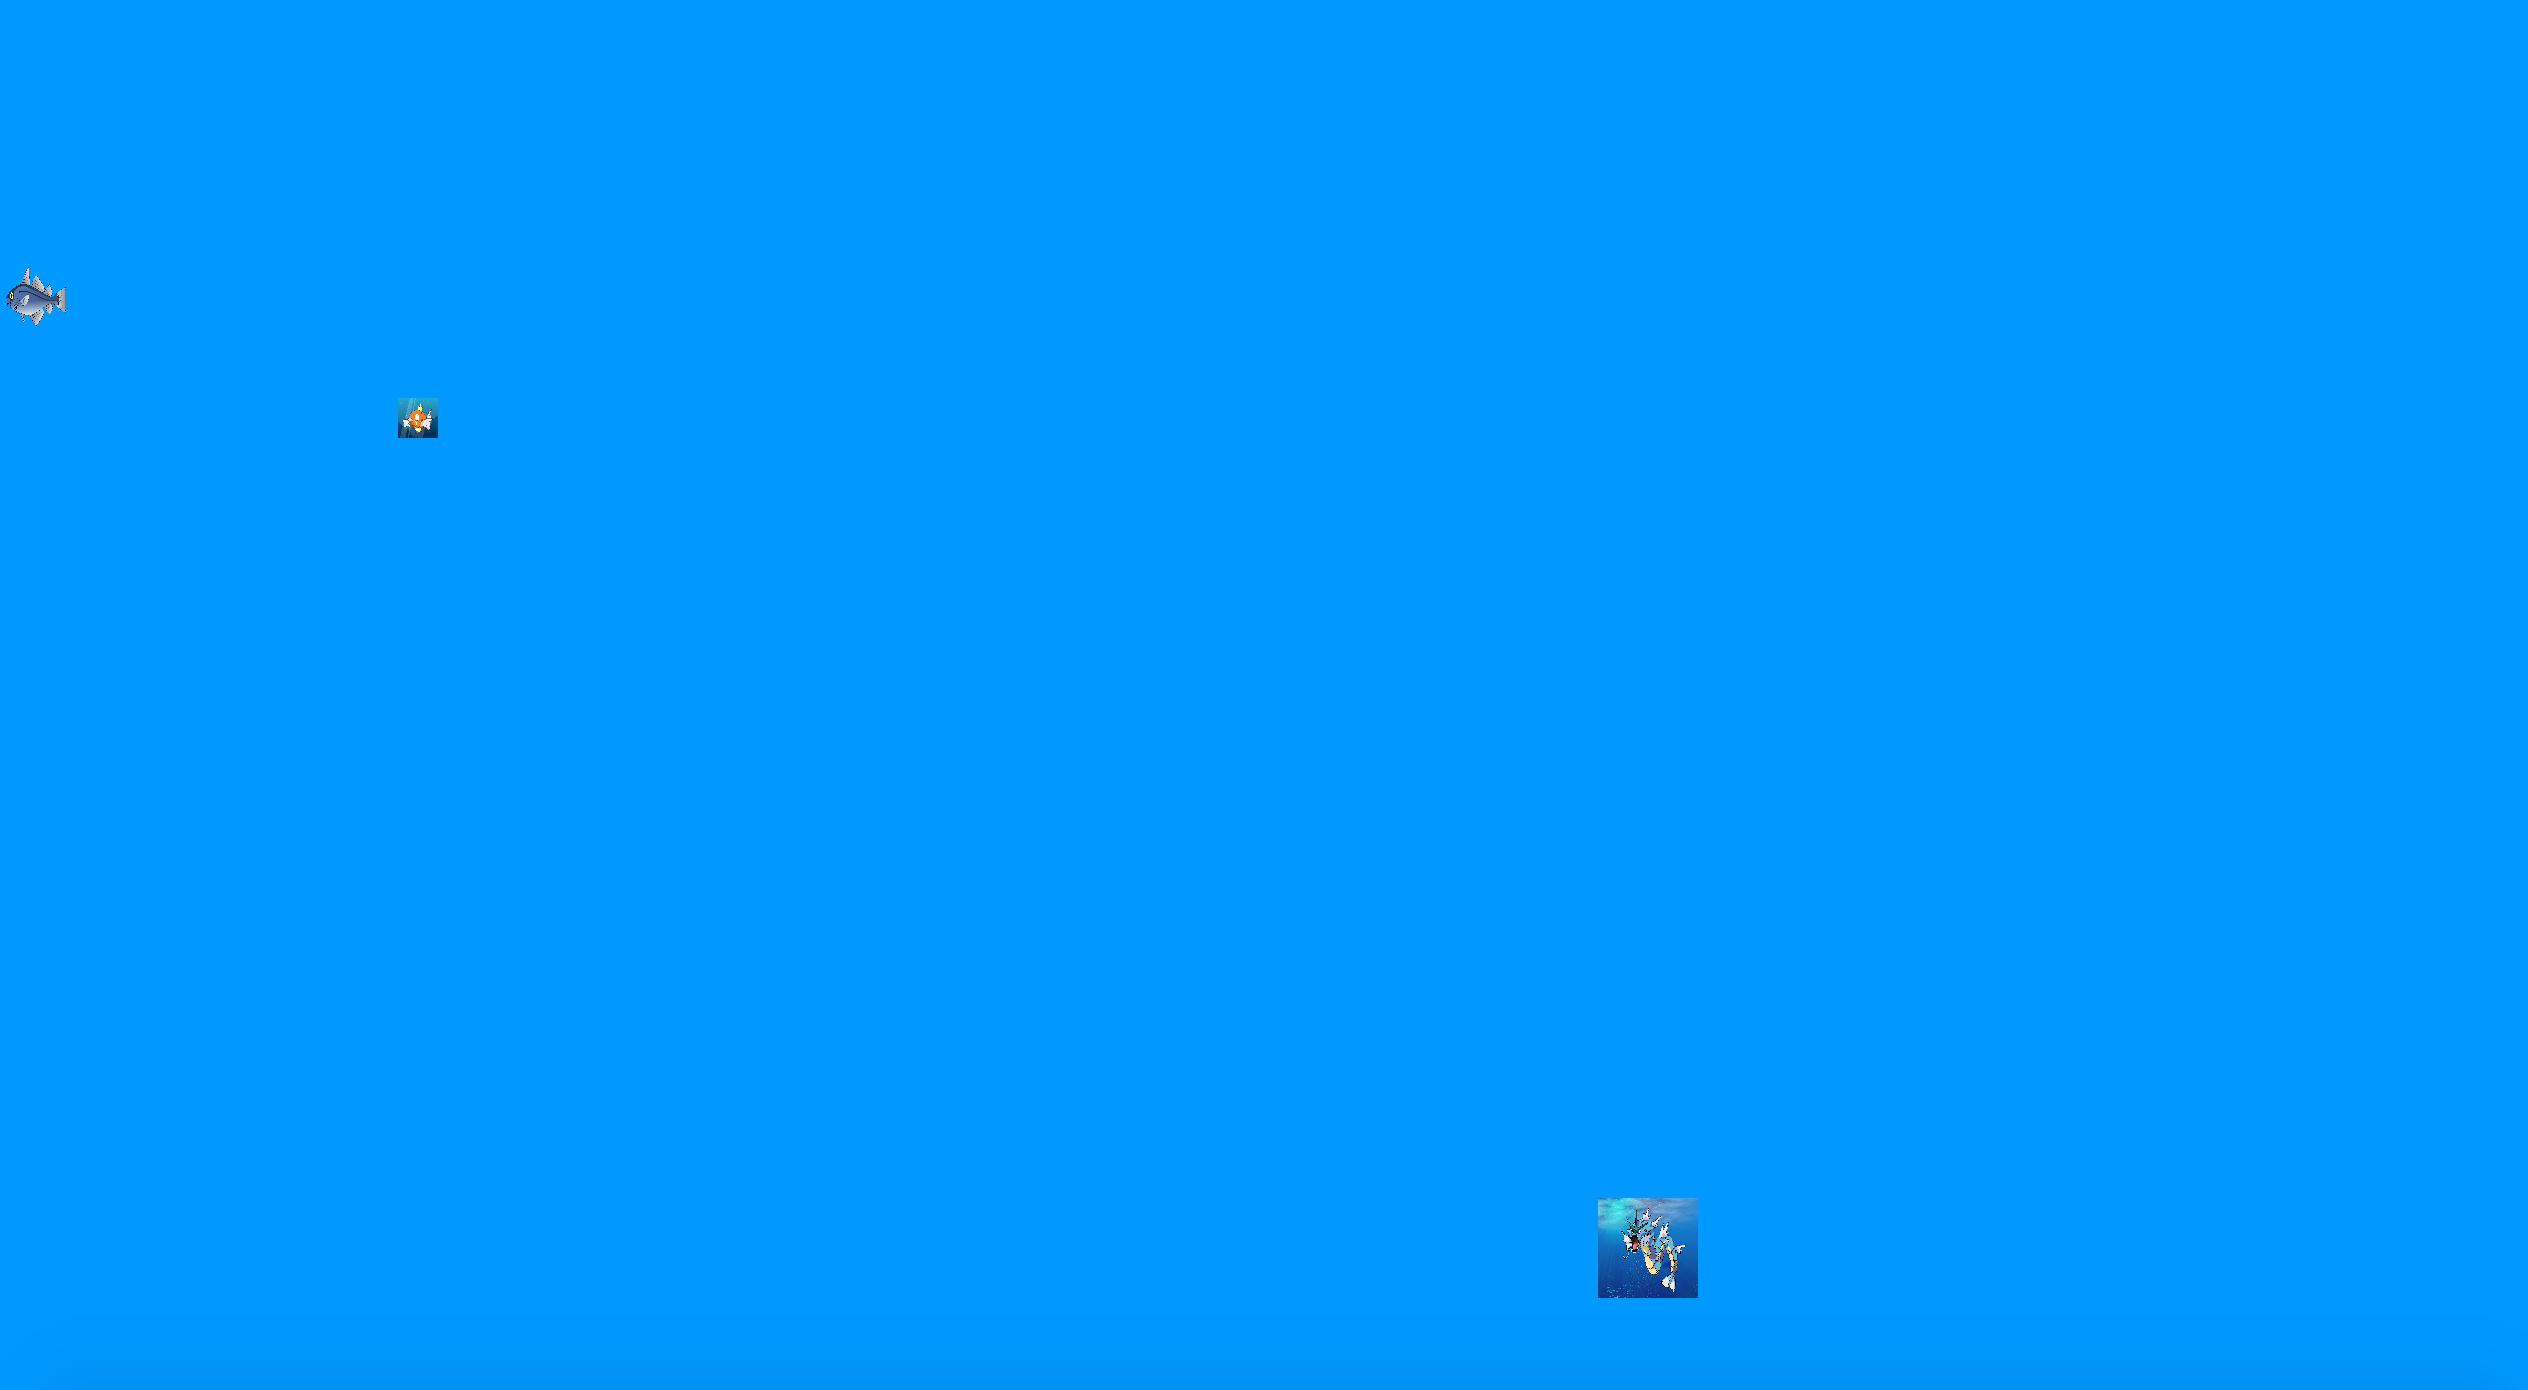
\includegraphics[scale=0.2]{Screenshot_Aqua}\end{center}
\end{figure}





\newpage
\section{Conclusion}

\indent Ce projet a été l'oeuvre d'une coopération de toute l'équipe. En effet nous avons dû mettre en pratique une architecture modèle-vue d'un côté
et contrôleur de l'autre. De plus, du côté contrôleur nous avons un client et un serveur, ce qui nous a permis de mettre
en pratique pour la première fois sur un projet concret nos connaissances de réseaux accumulées jusque là.\\
\indent Il a fallu réussir à emboîter la partie graphe, la partie serveur, la partie qui à la connaissance de l'état tous les
poissons, la partie client et la partie vue. Ce fût une grande épreuve, mais qui finalement s'est soldée par l'aboutissement
d'un aquarium fonctionnel (objet qui est d'ailleurs présent dans la plupart des foyers français. Qui n'a jamais rêvé de pouvoir
contrôler ses poissons en regardant son aquarium ?).\\
\indent Nous avons utilisé un large panel d'outils que nous avons appris ces dernières années : le langage C, Java, des connaissances en réseaux
mais aussi en système. L'entente au niveau de l'équipe a été cordiale : en effet chacun a travaillé professionellement sur
sa partie, et ce, de façon efficace. Le fait de rester assez proche du cahier des charges, afin d'essayer de satisfaire le client, nous
a permis d'éviter beaucoup de conflits lors de la fusion du travail de chacun.

%\end{doublespace}
%\input{besoinsf}
\end{document}
